\documentclass[letterpaper,11pt]{article}
\oddsidemargin -1.0cm \textwidth 17.5cm

\usepackage[utf8]{inputenc}
\usepackage[activeacute,spanish, es-lcroman]{babel}
\decimalpoint
\usepackage{amsfonts,setspace}
\usepackage{amsmath}
\usepackage{amssymb, amsmath, amsthm}
\usepackage{comment}
\usepackage{float}
\usepackage{amssymb}
\usepackage{dsfont}
\usepackage{anysize}
\usepackage{multicol}
\usepackage{enumerate}
\usepackage{graphicx}
\usepackage[left=1.5cm,top=2cm,right=1.5cm, bottom=1.7cm]{geometry}
\setlength\headheight{1.5em} 
\usepackage{fancyhdr}
\usepackage{multicol}
\usepackage{hyperref}
\usepackage{wrapfig}
\usepackage{subcaption}
\usepackage{siunitx}
\usepackage{cancel}
\usepackage{mdwlist}
\usepackage{svg}
\pagestyle{fancy}
\fancyhf{}
\renewcommand{\labelenumi}{\normalsize\bfseries P\arabic{enumi}.}
\renewcommand{\labelenumii}{\normalsize\bfseries (\alph{enumii})}
\renewcommand{\labelenumiii}{\normalsize\bfseries \roman{enumiii})}


\begin{document}

\fancyhead[L]{\itshape{Facultad de Ciencias F\'isicas y Matem\'aticas}}
\fancyhead[R]{\itshape{Universidad de Chile}}

\begin{minipage}{11.5cm}
    \begin{flushleft}
        \hspace*{-0.6cm}\textbf{FI1000-1 Introducción a la Física Clásica}\\
        \hspace*{-0.6cm}\textbf{Profesor:} Ignacio Bordeu\\
        \hspace*{-0.6cm}\textbf{Auxiliares:} Javier Cubillos \& Berenice Muruaga\\
        \hspace*{-0.6cm}\textbf{Auxiliares taller:} Pablo González \& Alejandro Cartes\\
    \end{flushleft}
\end{minipage}

\begin{picture}(2,3)
    \put(366, 10){
\includegraphics[scale=0.9]{2020-1/Imágenes/logo/dfi-fcfm.pdf}}
\end{picture}

\begin{center}
	\LARGE\textbf{Taller \#1}\\
	\Large{Trigonometría}
\end{center}

\vspace{-1cm}
\begin{enumerate}\setlength{\itemsep}{0.4cm}\addtocounter{enumi}{-1}

\rfoot[]{pág. \thepage}

\item[]

% \item Una tortuga se encuentra al pie de un cerro cuya inclinación es $\gamma$. Desde cierta posición avista, con un ángulo de elevación $\alpha$ respecto al piso, a su compañera tortuga que se encuentra en la punta de un poste vertical ubicado en la cima del cerro. Luego, la tortuga avanza una distancia $d$ en dirección al poste. En este lugar avista a su compañera con un ángulo de elevación $\beta$. Encuentre la altura $h$ del poste en el que se encuentra la compañera tortuga. Analice el caso $\gamma\rightarrow 0$

% \begin{figure}[H]
%     \centering
%     \svgpath{../../2021-2/img/aux1}
%     \includesvg[width=0.25\linewidth]{tortugas.svg}
% \end{figure}

\item Una persona ubicada en el punto $P$ (ver Figura P2) observa dos montañas, una a la izquierda y otra a la derecha. Sean $\alpha$ y $\beta$ los ángulos de elevación de estas montañas. Si la montaña de la izquierda tiene una altura $h$ y la separación entre las proyecciones de las cimas sobre el nivel de la superficie terrestre es $D$, calcule la altura del otro monte. 


\begin{figure}[H]
    \centering
    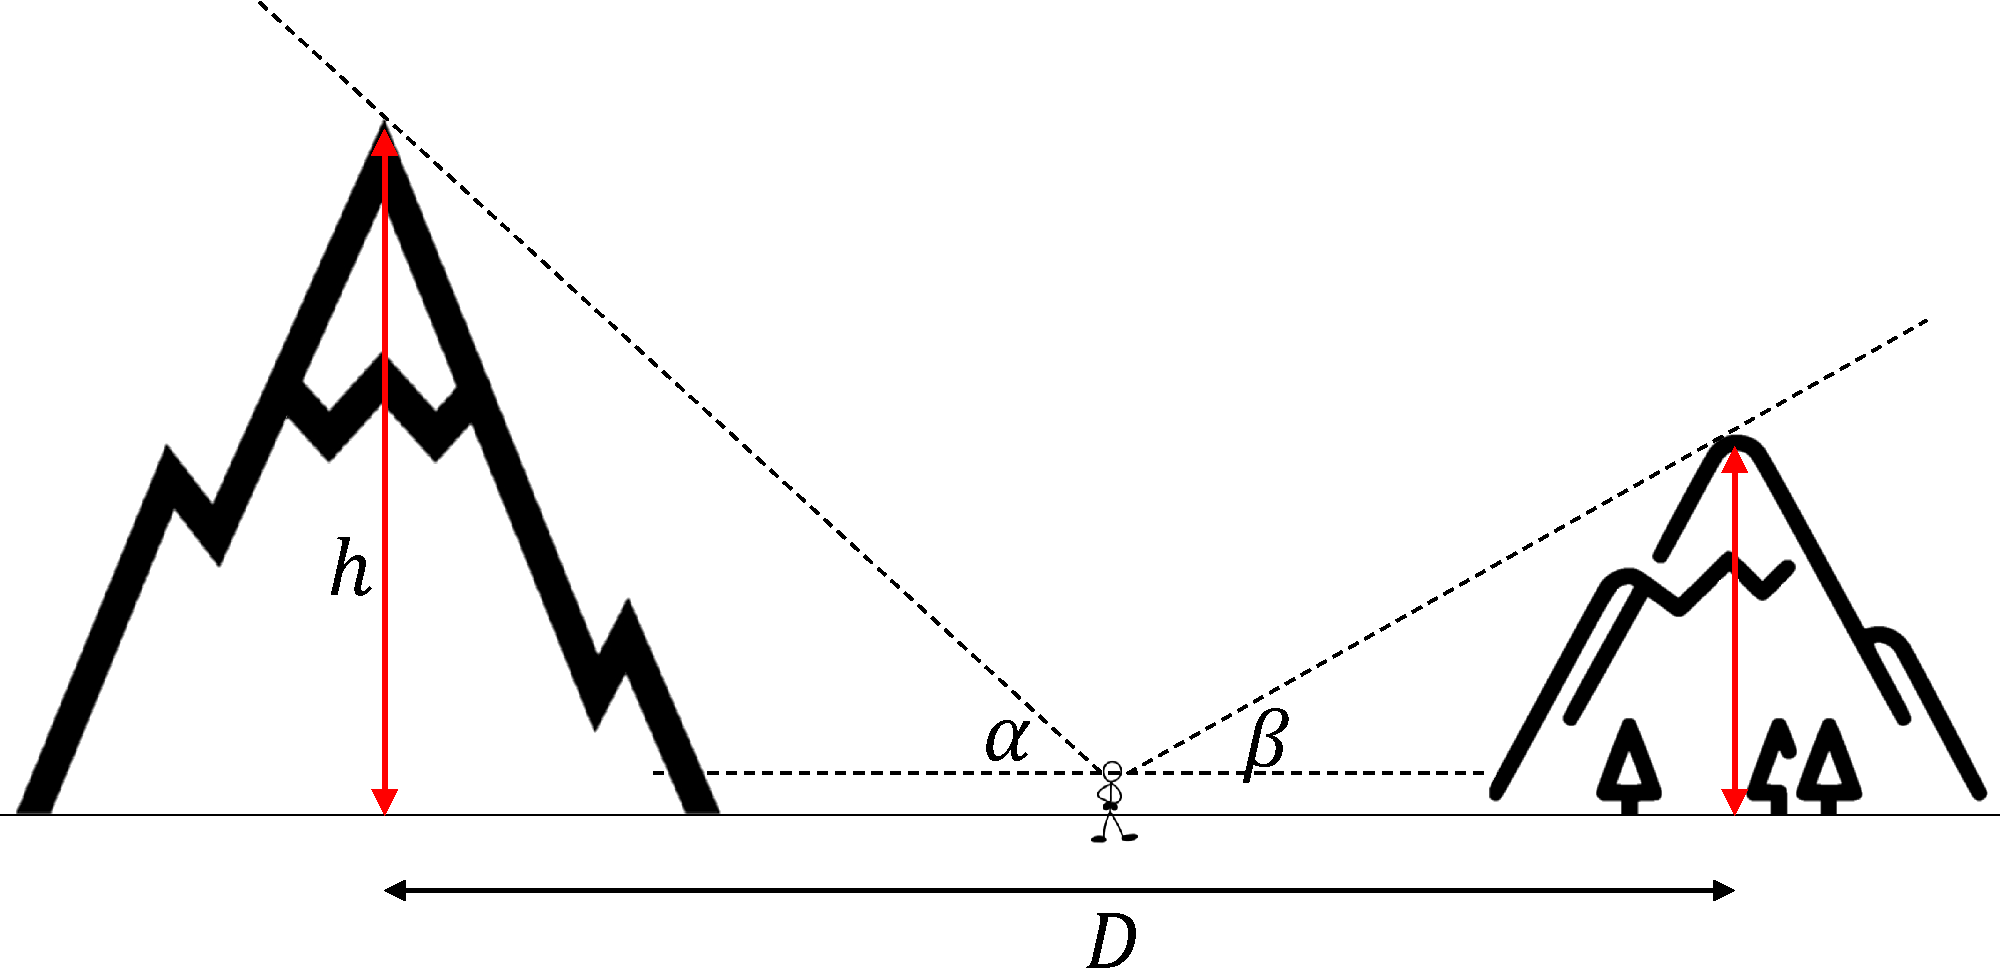
\includegraphics[width=0.4\linewidth]{2021-1/Imagenes/aux0/mountain.pdf}
\end{figure}


\item Considere la construcción de la figura, determine:

\begin{multicols}{2}
    \begin{figure}[H]
        \centering
        \includesvg[width=0.55\linewidth]{../../2022-1/img/aux0/sumaangulos.svg}
    \end{figure}
    \columnbreak
    \begin{enumerate}
        \item Los segmentos $\overline{EA}$, $\overline{ED}$, $\overline{DF}$, $\overline{OD}$ y $\overline{DB}$.\\
        Concluya que:
        $$\sin\left(\alpha+\beta\right)=\cos\alpha\sin\beta+\sin\alpha\cos\beta$$
        
        \item Los segmentos $\overline{OA}$, $\overline{OB}$ y $\overline{EF}$.\\
        Concluya que:
        $$\cos\left(\alpha+\beta\right)=\cos\alpha\cos\beta-\sin\alpha\sin\beta$$
    \end{enumerate}
\end{multicols}


\item Un terraplén de ferrocarril se levanta sobre un plano horizontal, y se requiere encontrar la distancia desde un punto A de dicho plano a un punto B de la parte superior del terraplén. Se escoge un punto C en el pie del terraplén (que esté en el mismo plano vertical que A y B), y se miden las distancias $AC$, $AB$ y el ángulo $\alpha = \angle BAC$. Si $AC = 14[m]$, $BC = 25 [m]$ y $\alpha = 21\degree$, calcular la medida del lado AB.\\


 \begin{figure}[H]
    \centering
     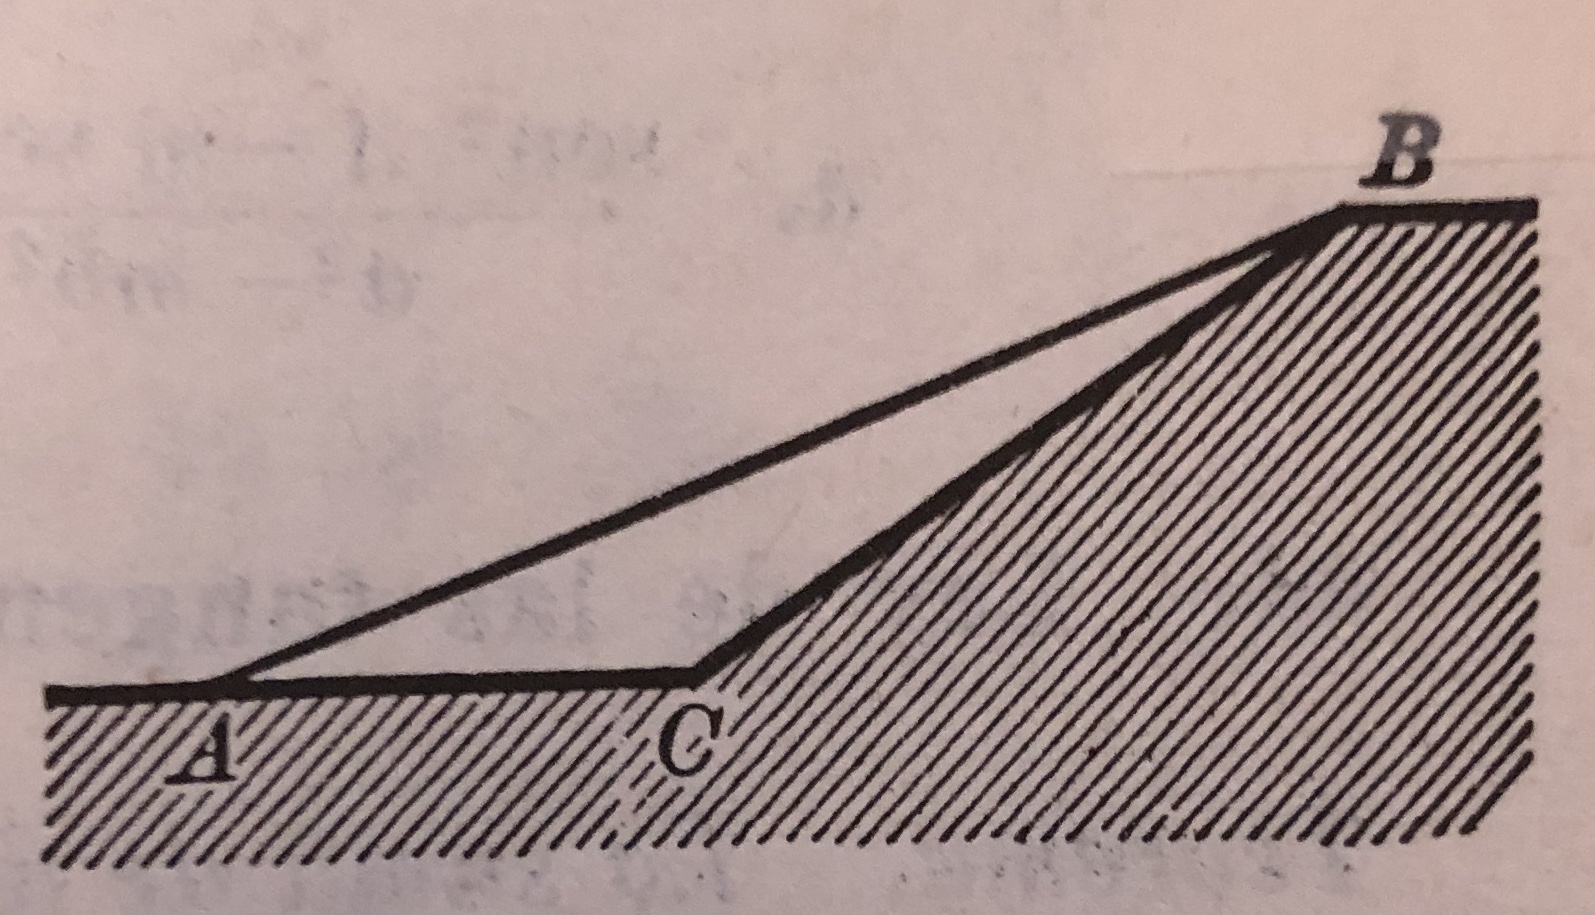
\includegraphics[height=5cm]{2022-2/Imagenes/t1p2.jpg}
 \end{figure}



% Para imágenes vectoriales -> el texto tiene que estar en LaTeX
% \begin{figure}[htbp]
%   \centering
%   \svgpath{../Imagenes/ejercicios}  -> .. irse pa'trás 
%   \includesvg{ej5.svg}
% \end{figure}

\end{enumerate}
\end{document}
